% =========================================================================
% MÓDULO 3: RESULTADOS EN 5 ETAPAS, TRAYECTORIAS Y SOTA (DIAPOSITIVAS 10 A 18)
% =========================================================================

% --- DIAPOSITIVA 10: MAPA GENERAL DE LAS CINCO ETAPAS EXPERIMENTALES ---
\begin{frame}{Dise\~no Experimental y Mapa de las Cinco Etapas}{Trazabilidad de los 723 entrenamientos bajo preprocesamiento fijo \texttt{P0} \cite{rodas_valencia_tpe_ecog}}
  \scriptsize
  \centering
  \renewcommand{\arraystretch}{1.28}
  \setlength{\tabcolsep}{4.5pt}
  \begin{tabularx}{\textwidth}{@{} l c c c c >{\raggedright\arraybackslash}X @{}}
    \toprule
    \rowcolor{ipnDark}
    \textcolor{white}{\textbf{Etapa Experimental (\texttt{P0} fijo)}} &
    \textcolor{white}{\textbf{S1}} &
    \textcolor{white}{\textbf{S2}} &
    \textcolor{white}{\textbf{S3}} &
    \textcolor{white}{\textbf{Media}} &
    \textcolor{white}{\textbf{Aporte e Interpretaci\'on Metodol\'ogica}} \\
    \midrule
    \textbf{1.\ \texttt{A0} Base (CV \'ep.\ 50)} & $0.4990$ & $0.4289$ & $0.7187$ & $\mathbf{0.5489}$ & L\'inea base inicial de referencia ($15$ fits). \\
    \rowcolor{rowLight}
    \textbf{2.\ \texttt{A5} sin TPE (CV \'ep.\ 50)} & $0.6038$ & $0.6216$ & $0.8258$ & $\mathbf{0.6837}$ & $\mathbf{+0.1349}$ por redise\~no arquitect\'onico ($14/15$ folds $>0$). \\
    \textbf{2b.\ \texttt{A5} sin TPE (\textit{Checkpoint*})} & $0.7103$ & $0.6466$ & $0.8422$ & $\mathbf{0.7330}$ & $\mathbf{+0.0493}$ por parada temprana sobre hist\'oricos sin TPE. \\
    \rowcolor{rowLight}
    \textbf{3.\ \texttt{A5} con TPE (Mejor trial CV)} & $0.7117$ & $0.6878$ & $0.8533$ & $\mathbf{0.7509}$ & $\mathbf{+0.0179}$ durante la b\'usqueda en Optuna ($480$ fits). \\
    \textbf{4.\ \texttt{A5} Verificada (Semillas nuevas)} & $0.6929$ & $0.6785$ & $0.8402$ & $\mathbf{0.7372}$ & $\mathbf{+0.0041}$ neto global vs.\ 2b; $\mathbf{+0.0319}$ en \texttt{S2} ($60$ fits). \\
    \midrule
    \rowcolor{rowLight}
    \textbf{5a.\ \texttt{A5} Test Inicial (\texttt{B1--B4})} & $0.6087$ & $0.5226$ & $0.7685$ & $\mathbf{0.6333}$ & Evaluaci\'on inicial en prueba con parada en \texttt{B5} ($9$ fits). \\
    \rowcolor{rowHighlight}
    \textbf{5b.\ \texttt{A5} Test Oficial (\texttt{B1--B5})} & $\mathbf{0.6723}$ & $\mathbf{0.5490}$ & $\mathbf{0.7796}$ & $\mathbf{0.6669}$ & $\mathbf{+0.0337}$ al reentrenar con los 5 bloques ($9/9 > 0$). \\
    \bottomrule
  \end{tabularx}
  \fuente{Creaci\'on propia a partir del protocolo experimental implementado en GitHub \cite{rodas_valencia_tpe_ecog}.}

  \takeaway{Todas las correlaciones se calculan sobre la trayectoria continua reconstruida con \textit{overlap-add}, promediando los 5 dedos, los 5 bloques en CV y las \textbf{3 semillas completas en Test} (\texttt{3042, 4042, 5042}) sin elegir la mejor semilla \cite{rodas_valencia_tpe_ecog}.}
\end{frame}

% --- DIAPOSITIVA 11: ETAPAS 1 Y 2: ABLACIONES ARQUITECTÓNICAS ---
\begin{frame}{Etapas 1 y 2: Campa\~na de Ablaciones Arquitect\'onicas}{Impacto cuantitativo de las variantes sobre 165 entrenamientos controlados \cite{rodas_valencia_tpe_ecog}}
  \begin{columns}[c,onlytextwidth]
    \begin{column}{0.40\textwidth}
      \begin{block}{Resultados Clave de Ablaci\'on}
        \scriptsize
        \begin{itemize}\setlength{\itemsep}{3.5pt}
          \item \textbf{Mayor salto interno ($\mathbf{+0.1349}$):} Pasar de \texttt{A0} ($0.5489$) a \texttt{A5} ($0.6837$) en \'epoca 50 mejora \textbf{$14$ de los $15$ pliegues} (\texttt{S2} gana $\mathbf{+0.1927}$; \'unica excepci\'on \texttt{S1-B3} con $-0.0359$).
          \item \textbf{Lecci\'on de \texttt{A3} ($0.5173$):} Usar \texttt{ConvTranspose1d} de forma aislada degrad\'o $-0.0316$. Su ventaja emerge solo al combinarse con \texttt{LayerNorm} (\texttt{A1}: $+0.0605$) y el nuevo orden del Decoder en \texttt{A5}.
          \item \textbf{Control experimental:} Se mantuvo fijo el preprocesamiento \texttt{P0} en las etapas posteriores para aislar sin confusi\'on el aporte de \texttt{A5} y TPE.
        \end{itemize}
      \end{block}
    \end{column}

    \begin{column}{0.57\textwidth}
      \centering
      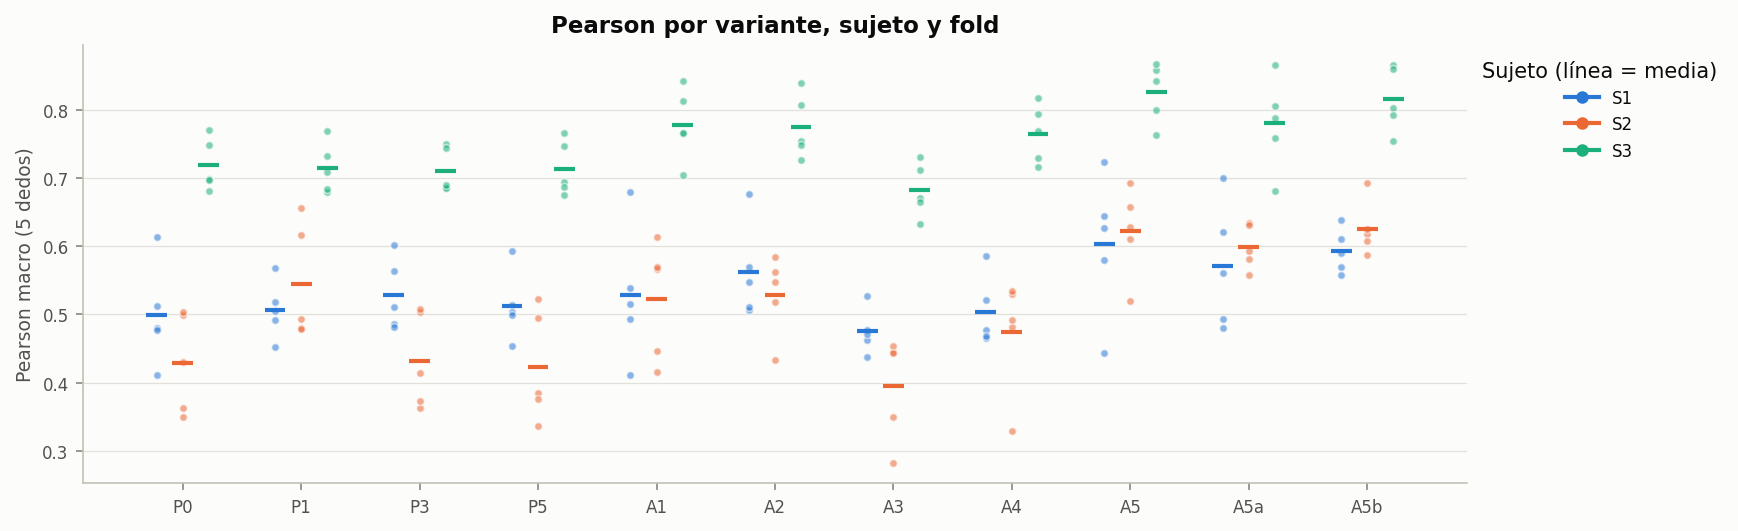
\includegraphics[width=\linewidth,height=0.49\textheight,keepaspectratio]{imgs/pearson_by_variant.png}
      \figcap{4}{Correlaci\'on de Pearson macro por variante (\texttt{P0--P5} y \texttt{A1--A5b}), sujeto y pliegue en la \'epoca 50. \textbf{Fuente:} Obtenida del repositorio GitHub \cite{rodas_valencia_tpe_ecog}.}
    \end{column}
  \end{columns}

  \takeaway{El redise\~no arquitect\'onico acoplado ($\texttt{A0} \to \texttt{A5}$) constituye el factor individual de mayor impacto en todo el proyecto, superando ampliamente el efecto posterior del ajuste fino de hiperpar\'ametros \cite{rodas_valencia_tpe_ecog}.}
\end{frame}

% --- DIAPOSITIVA 12: DINÁMICA DE CONVERGENCIA Y SELECCIÓN DE CHECKPOINT ---
\begin{frame}{Din\'amica de Convergencia y Selecci\'on de \textit{Checkpoint}}{Desacoplamiento del efecto de parada temprana ($+0.0493$) antes de aplicar Optuna TPE \cite{cawley2010overfitting,rodas_valencia_tpe_ecog}}
  \begin{columns}[c,onlytextwidth]
    \begin{column}{0.40\textwidth}
      \begin{block}{Puente Metodol\'ogico 2b}
        \scriptsize
        \begin{itemize}\setlength{\itemsep}{3.5pt}
          \item \textbf{Sobreajuste al final de las 50 \'epocas:} Las curvas de validaci\'on alcanzan su m\'aximo entre las \'epocas $18$ y $35$, degrad\'andose ligeramente hacia la \'epoca $50$.
          \item \textbf{Efecto puro del \textit{checkpoint} ($\mathbf{+0.0493}$):} Evaluar los mismos entrenamientos hist\'oricos de \texttt{A5} sin TPE con la regla de parada temprana ($\text{min}=15, \text{patience}=10$) eleva la media de $0.6837$ a $\mathbf{0.7330}$.
          \item \textbf{Impacto por sujeto:} \texttt{S1} sube $\mathbf{+0.1066}$ ($0.6038 \to 0.7103$), \texttt{S2} $+0.0250$ y \texttt{S3} $+0.0164$.
        \end{itemize}
      \end{block}
    \end{column}

    \begin{column}{0.57\textwidth}
      \centering
      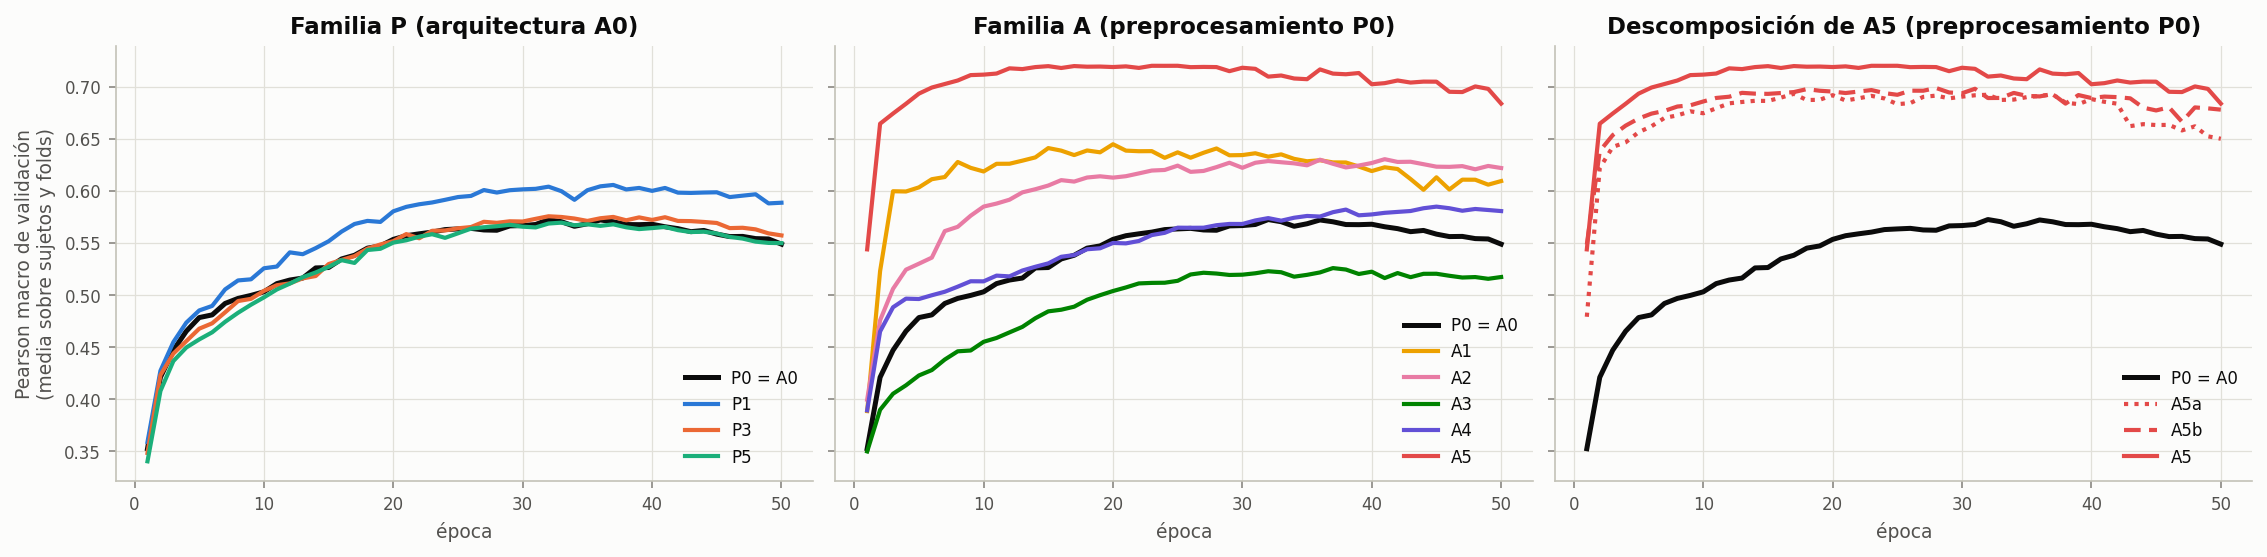
\includegraphics[width=\linewidth,height=0.52\textheight,keepaspectratio]{imgs/training_curves.png}
      \figcap{5}{Evoluci\'on de la correlaci\'on de validaci\'on por \'epoca para las familias \texttt{P}, \texttt{A} y la descomposici\'on hacia \texttt{A5}. \textbf{Fuente:} Obtenida del repositorio GitHub \cite{rodas_valencia_tpe_ecog}.}
    \end{column}
  \end{columns}

  \takeaway{Cuantificar este escal\'on de $\mathbf{+0.0493}$ evita un error metodol\'ogico com\'un: atribuir falsamente a la optimizaci\'on bayesiana una ganancia que en realidad proviene de seleccionar el mejor \textit{checkpoint} temporal \cite{cawley2010overfitting}.}
\end{frame}

% --- DIAPOSITIVA 13: ETAPAS 3 Y 4: BÚSQUEDA TPE Y VERIFICACIÓN MULTI-SEMILLA ---
\begin{frame}{Etapas 3 y 4: B\'usqueda TPE y Verificaci\'on Multi-Semilla}{Control del optimismo de b\'usqueda con 60 entrenamientos sobre semillas nuevas \cite{cawley2010overfitting,rodas_valencia_tpe_ecog}}
  \begin{columns}[c,onlytextwidth]
    \begin{column}{0.41\textwidth}
      \begin{block}{Auditor\'ia Estad\'istica de TPE}
        \scriptsize
        \begin{itemize}\setlength{\itemsep}{3pt}
          \item \textbf{Etapa 3 (Mejor Trial TPE = $\mathbf{0.7509}$):} Frente a \texttt{A5} con \textit{checkpoint} ($0.7330$), la b\'usqueda aporta $\mathbf{+0.0179}$ en la media ($\text{S2}$ sube $+0.0413$).
          \item \textbf{Etapa 4 (Verificaci\'on con 2 semillas nuevas/fold = $60$ fits):}
            \begin{itemize}\scriptsize
              \item \textbf{\texttt{A5} ($\mathbf{0.7372}$) supera a \texttt{A5b} ($0.7112$)} por $\mathbf{+0.0260}$ con mejoras en los 3 sujetos.
              \item Al descontar el sesgo del m\'aximo \cite{cawley2010overfitting}, la ganancia global sobre $0.7330$ es marginal ($\mathbf{+0.0041}$), pero \textbf{se mantiene un beneficio real en \texttt{S2} ($\mathbf{+0.0319}$)}.
            \end{itemize}
        \end{itemize}
      \end{block}
    \end{column}

    \begin{column}{0.56\textwidth}
      \centering
      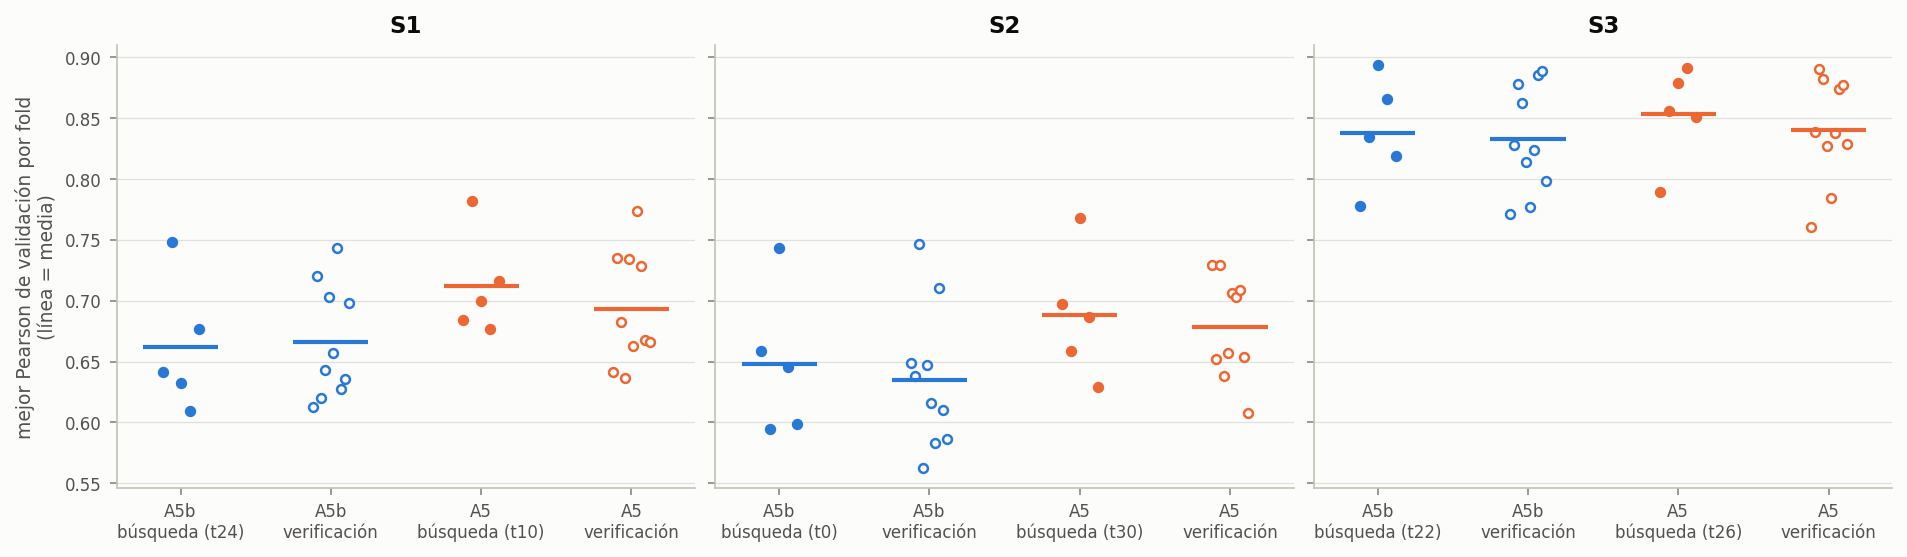
\includegraphics[width=\linewidth,height=0.52\textheight,keepaspectratio]{imgs/verification.png}
      \figcap{6}{Contraste entre el puntaje de b\'usqueda TPE y la verificaci\'on con semillas independientes para \texttt{A5} y \texttt{A5b} en los 3 sujetos. \textbf{Fuente:} Obtenida del repositorio GitHub \cite{rodas_valencia_tpe_ecog}.}
    \end{column}
  \end{columns}

  \takeaway{La verificaci\'on multi-semilla demostr\'o que \texttt{S1} y \texttt{S3} ya operaban cerca de su techo con hiperpar\'ametros base, mientras que TPE fue determinante para rescatar el desempe\~no del \textbf{Sujeto 2} ($+0.0319$) y confirmar la superioridad de \texttt{A5} sobre \texttt{A5b} \cite{rodas_valencia_tpe_ecog}.}
\end{frame}

% --- DIAPOSITIVA 14: CONFIGURACIONES SELECCIONADAS Y REGLA DE ÉPOCAS FIJAS ---
\begin{frame}{Configuraciones Seleccionadas por Sujeto y Regla de \'Epocas Fijas}{Modelos ganadores de la familia \texttt{A5} y protocolo de transici\'on al conjunto de prueba \cite{rodas_valencia_tpe_ecog}}
  \scriptsize
  \centering
  \renewcommand{\arraystretch}{1.35}
  \setlength{\tabcolsep}{5.5pt}
  \begin{tabularx}{\textwidth}{@{} l c c c c c c >{\raggedright\arraybackslash}X @{}}
    \toprule
    \rowcolor{ipnDark}
    \textcolor{white}{\textbf{Sujeto}} &
    \textcolor{white}{\textbf{Trial}} &
    \textcolor{white}{\textbf{Kernel $k$}} &
    \textcolor{white}{\textbf{Niveles $L$}} &
    \textcolor{white}{\textbf{Canales $f$}} &
    \textcolor{white}{\textbf{Par\'ametros}} &
    \textcolor{white}{\textbf{Verif.\ CV}} &
    \textcolor{white}{\textbf{Horizonte Fijo Test (\texttt{B1--B5})}} \\
    \midrule
    \textbf{\texttt{S1}} & Trial 10 & $k = 5$ & $L = 5$ & $f = 64$ & $\mathbf{9.35\text{ M}}$ & $0.6929 \pm 0.0566$ & $\mathbf{21\text{ \'epocas}}$ ($\eta = 1.38\times 10^{-4}$) \\
    \rowcolor{rowHighlight}
    \textbf{\texttt{S2}} & Trial 30 & $k = 7$ & $L = 5$ & $f = 96$ & $\mathbf{28.03\text{ M}}$ & $0.6785 \pm 0.0680$ & $\mathbf{32\text{ \'epocas}}$ ($\eta = 5.16\times 10^{-5}$) \\
    \textbf{\texttt{S3}} & Trial 26 & $k = 7$ & $L = 5$ & $f = 64$ & $\mathbf{12.71\text{ M}}$ & $0.8402 \pm 0.0369$ & $\mathbf{28\text{ \'epocas}}$ ($\eta = 5.10\times 10^{-5}$) \\
    \midrule
    \rowcolor{rowLight}
    \textbf{Media} & --- & --- & --- & --- & $16.70\text{ M}$ & $\mathbf{0.7372}$ & Mediana de $10$ corridas de verif. \\
    \bottomrule
  \end{tabularx}
  \fuente{Creaci\'on propia, obtenida del repositorio GitHub \cite{rodas_valencia_tpe_ecog}.}

  \vspace{1.5mm}
  \begin{columns}[T,onlytextwidth]
    \begin{column}{0.48\textwidth}
      \begin{block}{Protocolo Inicial \texttt{b1b4\_es\_b5}}
        \scriptsize
        Entrena sobre los bloques \texttt{B1--B4} ($80\%$ de los datos) y utiliza el bloque \texttt{B5} como validaci\'on interna para parada temprana. Desaprovecha el bloque m\'as cercano al conjunto de prueba.
      \end{block}
    \end{column}
    \begin{column}{0.48\textwidth}
      \begin{alertblock}{Protocolo Reentrenado \texttt{b1b5\_fixed}}
        \scriptsize
        Integra el $\mathbf{100\%}$ \textbf{de los bloques de desarrollo (\texttt{B1--B5})} entrenando durante la mediana exacta de \'epocas verificadas ($21, 32\text{ y }28$), sin observar jam\'as el bloque de prueba oficial.
      \end{alertblock}
    \end{column}
  \end{columns}
\end{frame}

% --- DIAPOSITIVA 15: ETAPA 5: EVALUACIÓN EN EL CONJUNTO DE PRUEBA OFICIAL ---
\begin{frame}{Etapa 5: Evaluaci\'on en el Conjunto de Prueba Oficial}{Desempe\~no final auditado sobre las tres semillas independientes (\texttt{3042, 4042, 5042}) \cite{lin1989concordance,rodas_valencia_tpe_ecog}}
  \begin{columns}[c,onlytextwidth]
    \begin{column}{0.49\textwidth}
      \scriptsize
      \centering
      \renewcommand{\arraystretch}{1.24}
      \setlength{\tabcolsep}{2.8pt}
      \begin{tabular}{@{} l c c c c @{}}
        \toprule
        \rowcolor{ipnDark}
        \textcolor{white}{\textbf{Suj.}} &
        \textcolor{white}{\textbf{\texttt{B1--B4}}} &
        \textcolor{white}{\textbf{\texttt{B1--B5} (Test)}} &
        \textcolor{white}{\textbf{CCC}} &
        \textcolor{white}{\textbf{MSE}} \\
        \midrule
        \textbf{\texttt{S1}} & $0.6087$ & $\mathbf{0.6723 \pm 0.0009}$ & $0.5534$ & $0.6497$ \\
        \rowcolor{rowLight}
        \textbf{\texttt{S2}} & $0.5226$ & $\mathbf{0.5490 \pm 0.0143}$ & $0.4050$ & $0.8667$ \\
        \textbf{\texttt{S3}} & $0.7685$ & $\mathbf{0.7796 \pm 0.0069}$ & $0.7694$ & $0.3606$ \\
        \midrule
        \rowcolor{rowHighlight}
        \textbf{Media} & $\mathbf{0.6333}$ & $\mathbf{0.6669}$ ($\mathbf{+0.0337}$) & $\mathbf{0.5759}$ & $\mathbf{0.6257}$ \\
        \bottomrule
      \end{tabular}
      \fuente{Creaci\'on propia, obtenida del repositorio GitHub \cite{rodas_valencia_tpe_ecog}.}

      \vspace{1.2mm}
      \begin{block}{Consistencia en las 9 Ejecuciones}
        \scriptsize
        \begin{itemize}\setlength{\itemsep}{2pt}
          \item El protocolo \texttt{b1b5\_fixed} supera a \texttt{b1b4\_es\_b5} en las \textbf{$9/9$ parejas sujeto-semilla} ($+0.0635$ en \texttt{S1}, $+0.0264$ en \texttt{S2}, $+0.0111$ en \texttt{S3}).
          \item Mejora simult\'aneamente el $\operatorname{CCC}$ de Lin ($0.5210 \to \mathbf{0.5759}$) y reduce el $\operatorname{MSE}$ ($0.6597 \to \mathbf{0.6257}$) \cite{lin1989concordance}.
        \end{itemize}
      \end{block}
    \end{column}

    \begin{column}{0.48\textwidth}
      \centering
      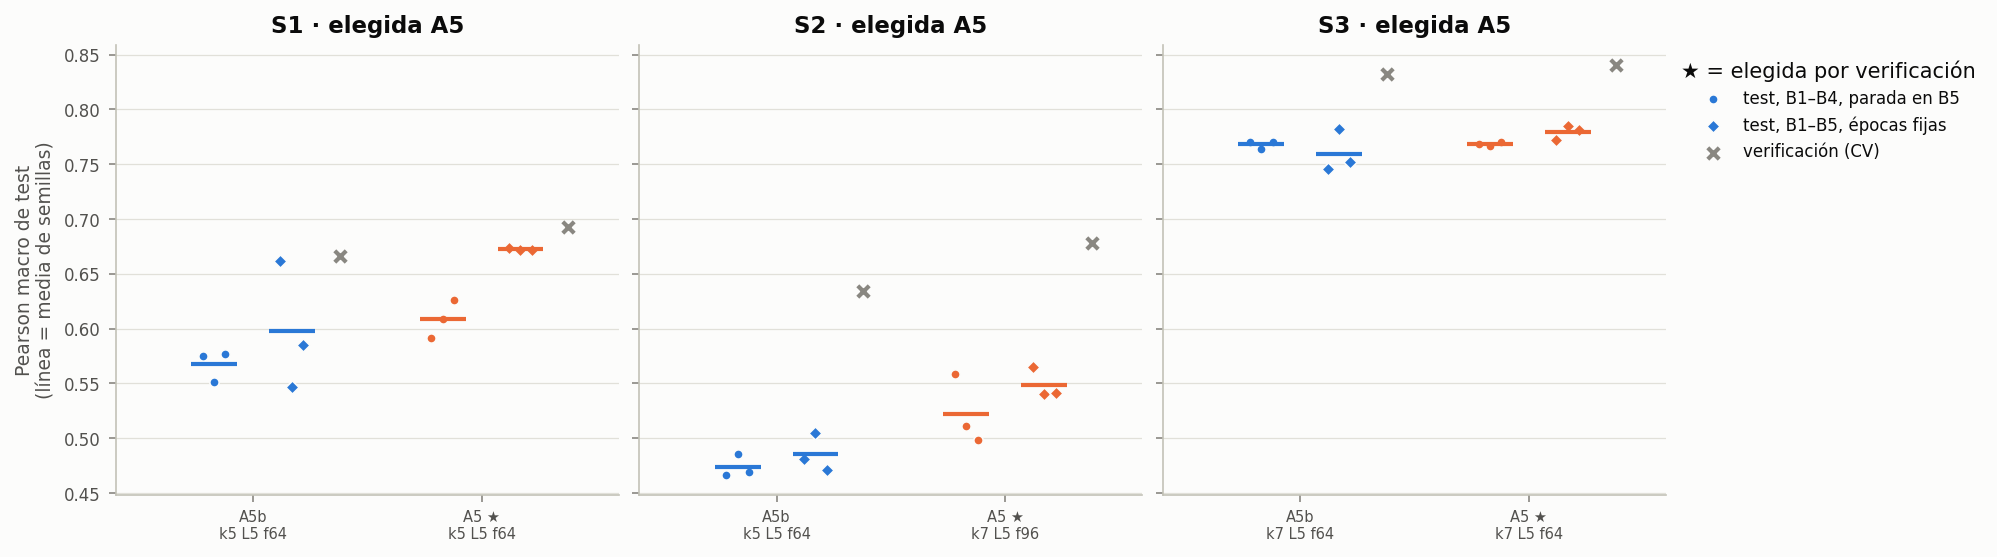
\includegraphics[width=\linewidth,height=0.50\textheight,keepaspectratio]{imgs/test_scores.png}
      \figcap{7}{Puntajes en el conjunto de prueba oficial por sujeto y semilla: protocolo inicial (\texttt{B1--B4}) frente a reentrenamiento completo (\texttt{B1--B5}). \textbf{Fuente:} Obtenida del repositorio GitHub \cite{rodas_valencia_tpe_ecog}.}
    \end{column}
  \end{columns}

  \takeaway{Por transparencia metodol\'ogica se reportan siempre ambas cifras: $0.6333$ como primera evaluaci\'on en prueba y $\mathbf{0.6669}$ como resultado del protocolo reentrenado sobre los 5 bloques \cite{rodas_valencia_tpe_ecog}.}
\end{frame}

% --- DIAPOSITIVA 16: ANÁLISIS DE RESULTADOS POR SUJETO Y POR DEDO ---
\begin{frame}{An\'alisis de Resultados por Sujeto y por Dedo}{Desempe\~no individual de los cinco dedos e interpretaci\'on biomec\'anica \cite{rodas_valencia_tpe_ecog}}
  \begin{columns}[c,onlytextwidth]
    \begin{column}{0.46\textwidth}
      \scriptsize
      \centering
      \renewcommand{\arraystretch}{1.22}
      \setlength{\tabcolsep}{3.2pt}
      \begin{tabular}{@{} l c c c c @{}}
        \toprule
        \rowcolor{ipnDark}
        \textcolor{white}{\textbf{Dedo}} &
        \textcolor{white}{\textbf{S1}} &
        \textcolor{white}{\textbf{S2}} &
        \textcolor{white}{\textbf{S3}} &
        \textcolor{white}{\textbf{Media Test}} \\
        \midrule
        \rowcolor{rowHighlight}
        \textbf{1.\ Anular} & $0.7429$ & $0.6431$ & $0.7745$ & $\mathbf{0.7202}$ \\
        \rowcolor{rowLight}
        \textbf{2.\ \'Indice} & $0.7525$ & $0.6197$ & $0.7760$ & $\mathbf{0.7161}$ \\
        \textbf{3.\ Pulgar} & $0.6777$ & $0.5835$ & $0.8130$ & $\mathbf{0.6914}$ \\
        \rowcolor{rowLight}
        \textbf{4.\ Me\~nique} & $0.6085$ & $0.4918$ & $0.7982$ & $\mathbf{0.6328}$ \\
        \textbf{5.\ Medio} & $0.5798$ & $0.4107$ & $0.7322$ & $\mathbf{0.5742}$ \\
        \midrule
        \textbf{Media Sujeto} & $\mathbf{0.6723}$ & $\mathbf{0.5490}$ & $\mathbf{0.7796}$ & $\mathbf{0.6669}$ \\
        \bottomrule
      \end{tabular}
      \fuente{Creaci\'on propia, obtenida del repositorio GitHub \cite{rodas_valencia_tpe_ecog}.}

      \vspace{1.5mm}
      \begin{block}{Patr\'on Somatot\'opico y Biomec\'anico}
        \scriptsize
        \begin{itemize}\setlength{\itemsep}{2pt}
          \item \textbf{Anular ($0.7202$) e \'Indice ($0.7161$)} presentan la mayor fidelidad de reconstrucci\'on en los 3 sujetos.
          \item El \textbf{dedo Medio ($0.5742$)} constituye el mayor reto ($\text{S2}=0.4107$) por su fuerte coactivaci\'on tendinosa y solapamiento cortical con los dedos adyacentes.
        \end{itemize}
      \end{block}
    \end{column}

    \begin{column}{0.51\textwidth}
      \centering
      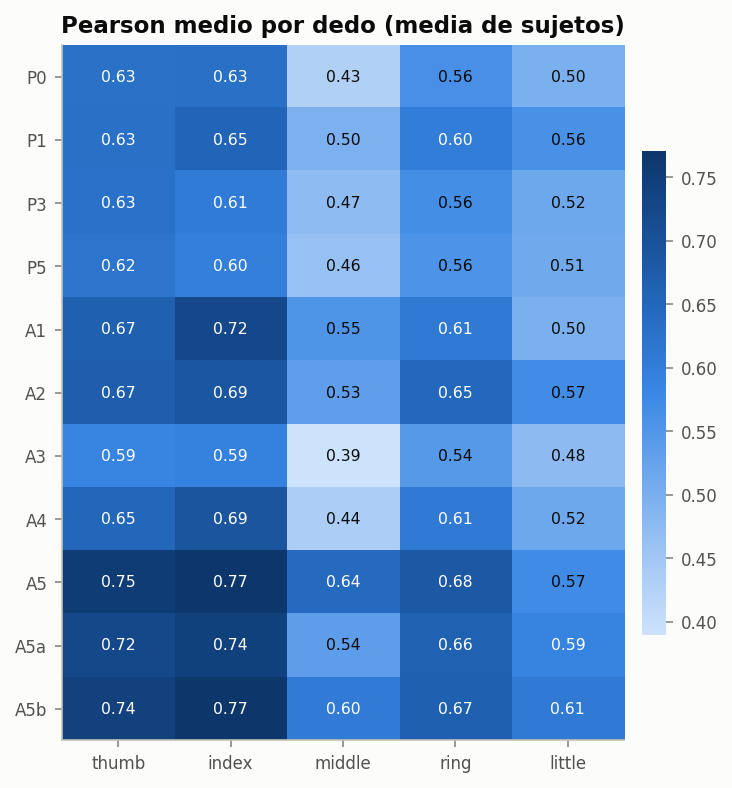
\includegraphics[width=\linewidth,height=0.52\textheight,keepaspectratio]{imgs/pearson_per_finger.png}
      \figcap{8}{Mapa de calor de correlaci\'on de Pearson por dedo a trav\'es de las variantes evaluadas (media de los tres sujetos). \textbf{Fuente:} Obtenida del repositorio GitHub \cite{rodas_valencia_tpe_ecog}.}
    \end{column}
  \end{columns}
\end{frame}

% --- DIAPOSITIVA 17: DEMOSTRACIÓN DE TRAYECTORIAS CONTINUAS Y AUDITORÍA V01-V14 ---
\begin{frame}{Demostraci\'on de Trayectorias Continuas y Auditor\'ia \texttt{V01--V14}}{Comparaci\'on visual del seguimiento cinem\'atico y verificaci\'on de integridad del software \cite{rodas_valencia_tpe_ecog}}
  \begin{columns}[T,onlytextwidth]
    \begin{column}{0.48\textwidth}
      \centering
      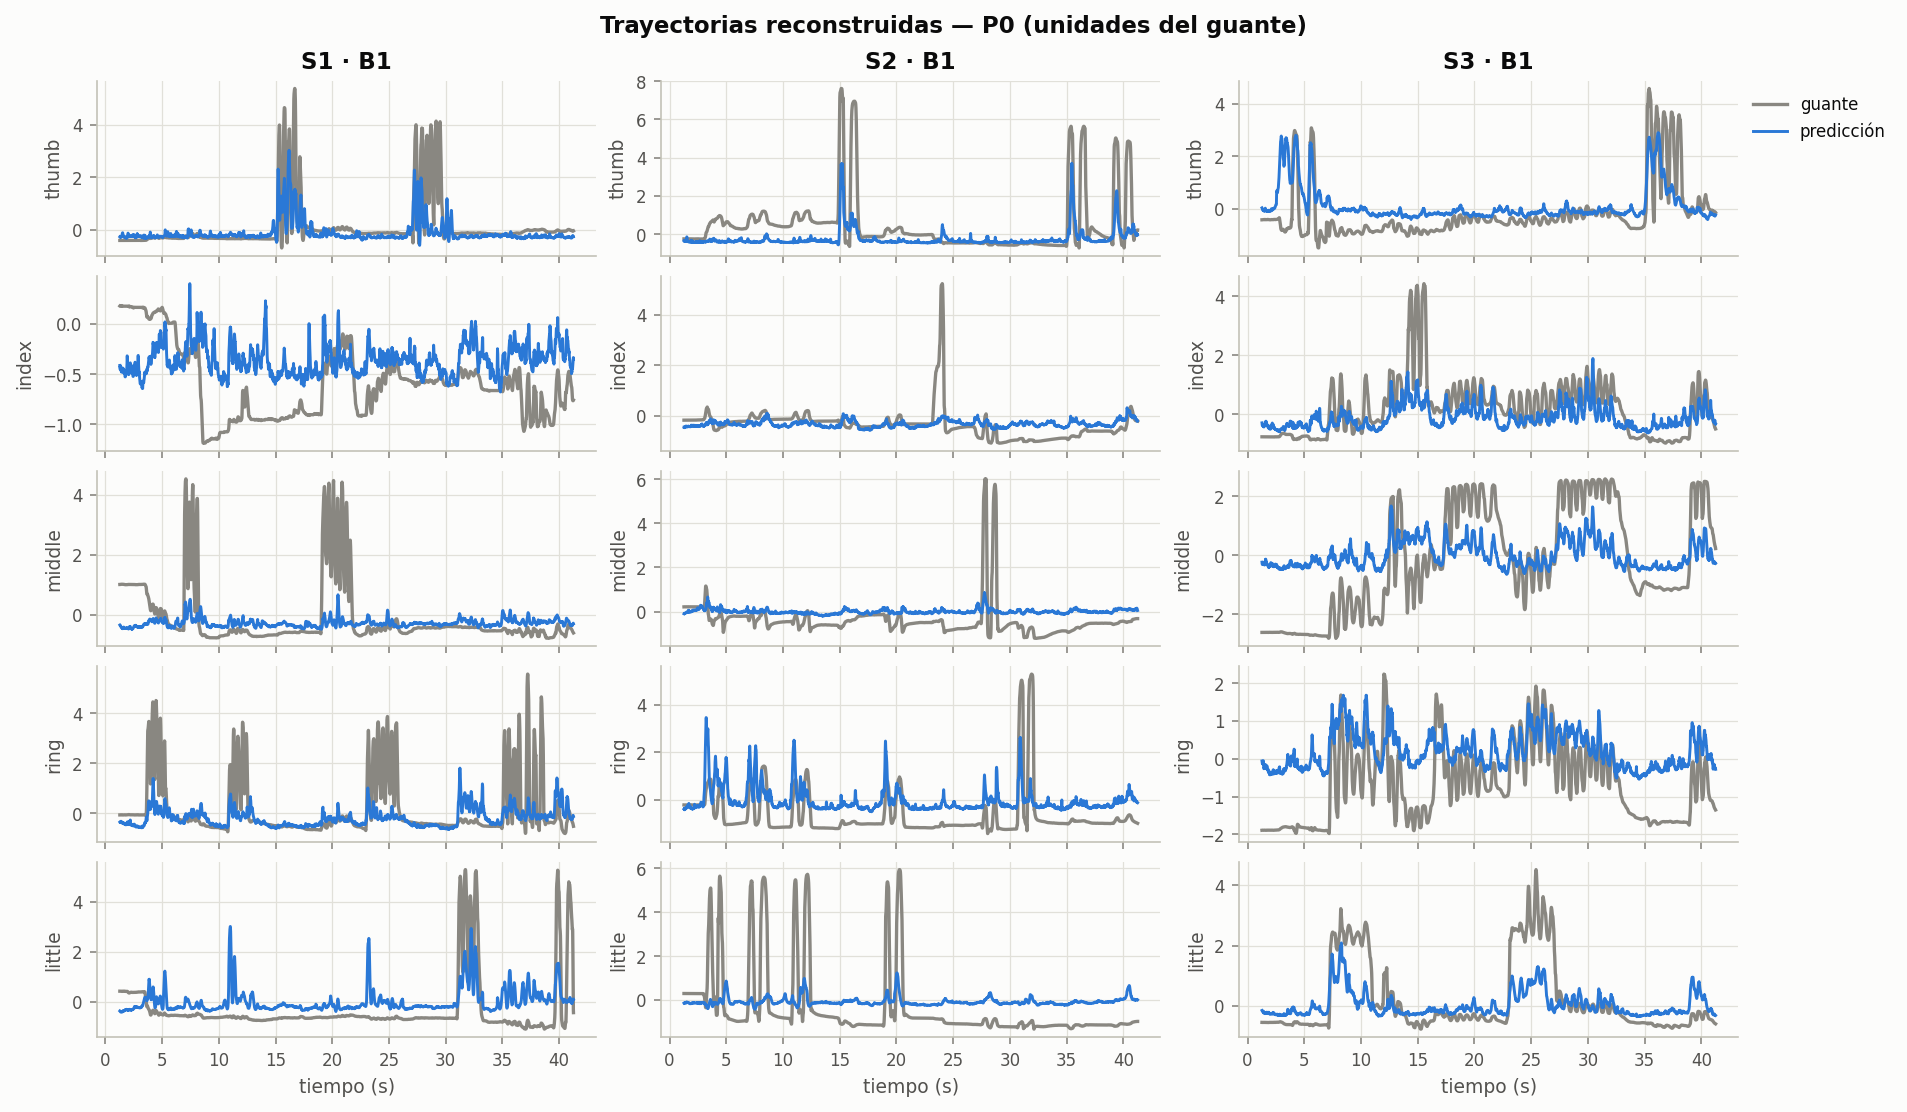
\includegraphics[width=\linewidth,height=0.45\textheight,keepaspectratio]{imgs/example_predictions_P0.png}
      \figcap{9}{\textbf{Modelo Base \texttt{A0/P0} ($0.5489$ CV):} predicciones con oscilaciones espurias. \textbf{Fuente:} Obtenida del repositorio GitHub \cite{rodas_valencia_tpe_ecog}.}
    \end{column}
    \begin{column}{0.48\textwidth}
      \centering
      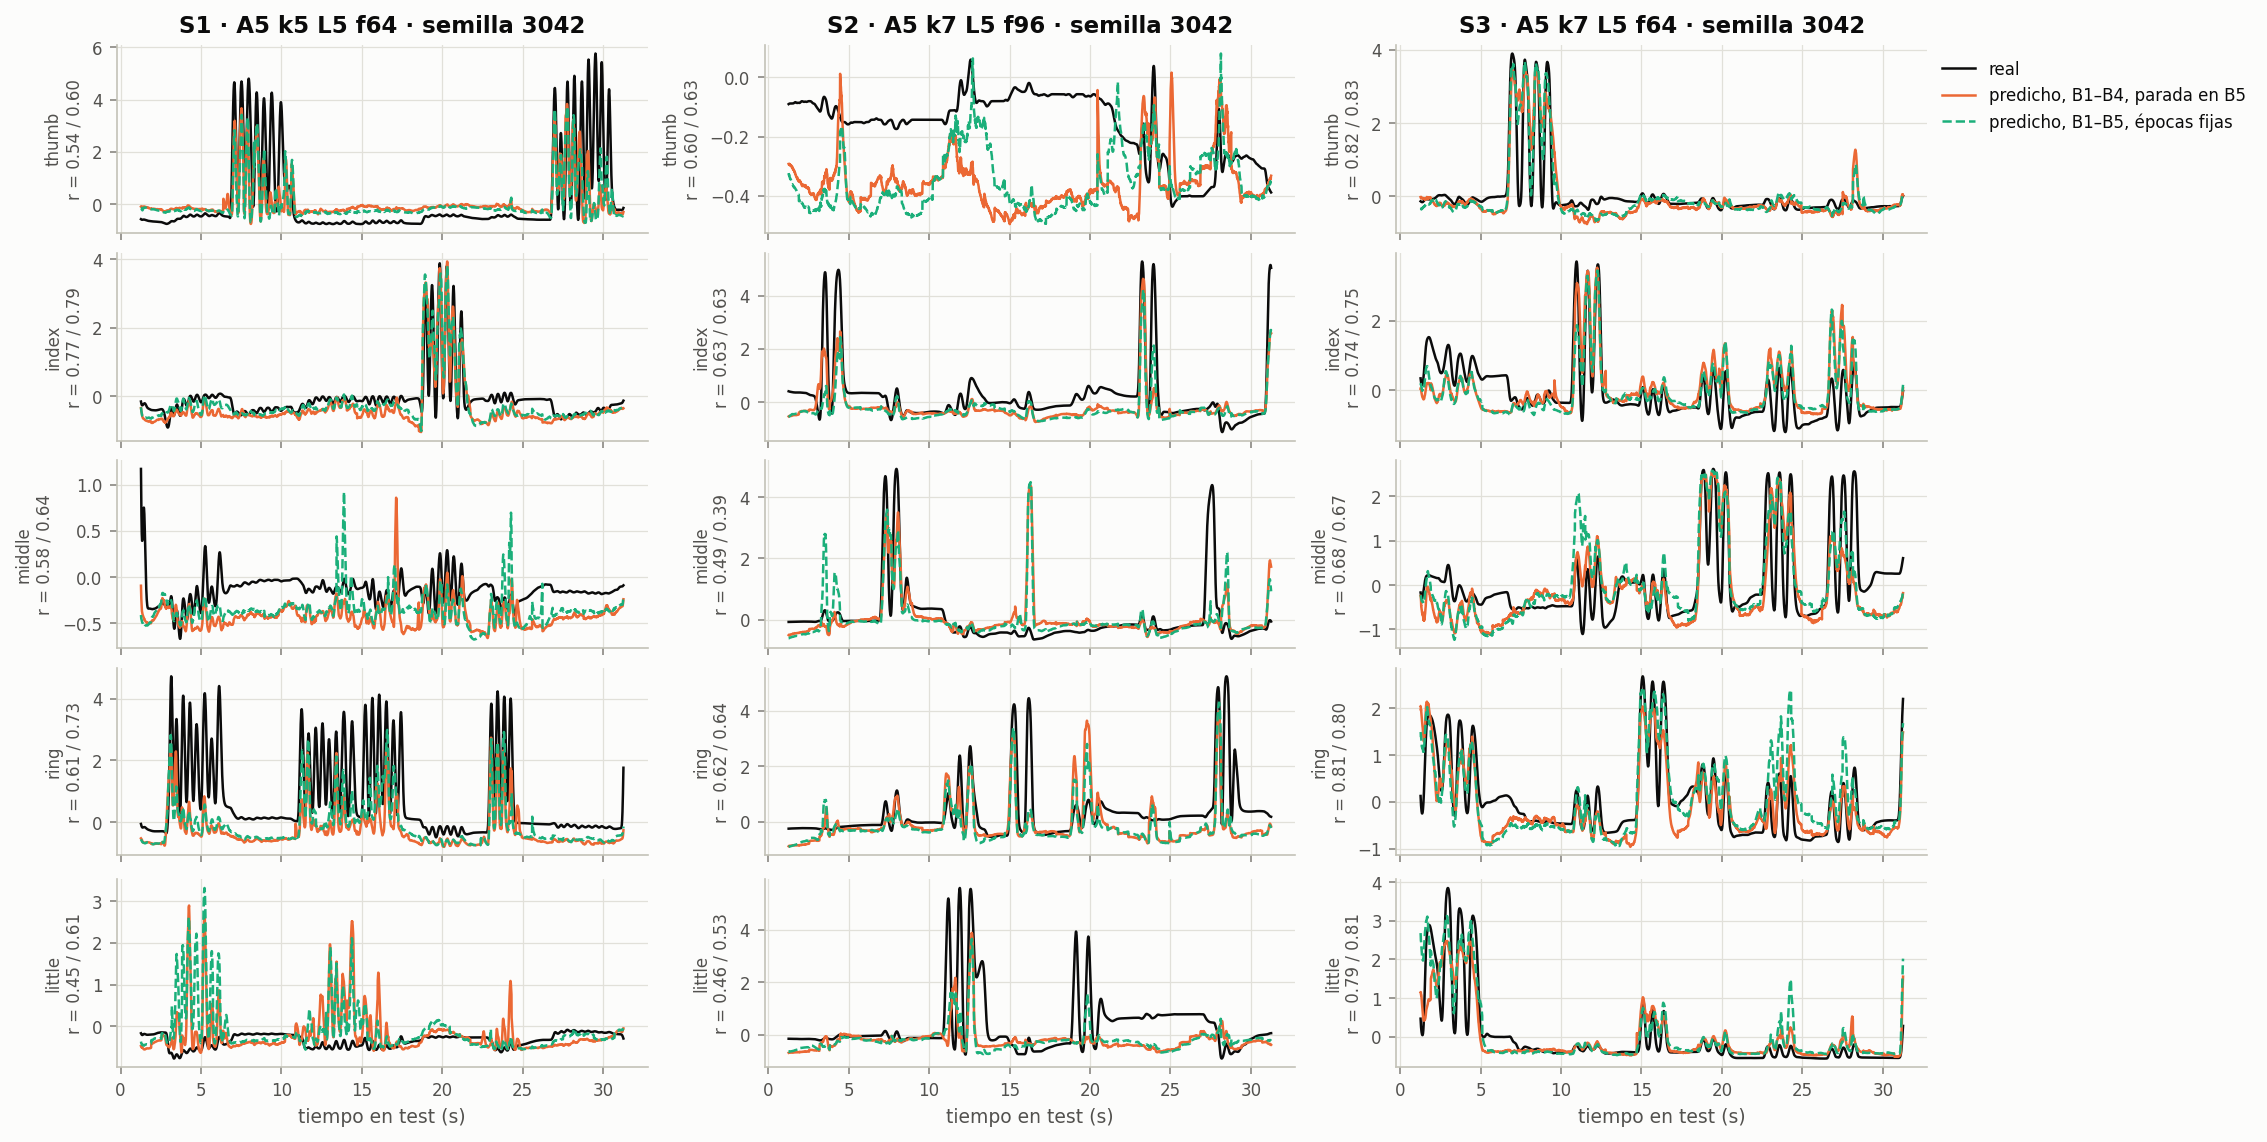
\includegraphics[width=\linewidth,height=0.45\textheight,keepaspectratio]{imgs/test_trajectories.png}
      \figcap{10}{\textbf{Modelo Final \texttt{A5} en Test Oficial ($0.6669$):} seguimiento preciso de flexi\'on y reposo. \textbf{Fuente:} Obtenida del repositorio GitHub \cite{rodas_valencia_tpe_ecog}.}
    \end{column}
  \end{columns}

  \takeaway{\textbf{Auditor\'ia Automatizada (\texttt{14/14 PASS}):} Las compuertas \texttt{V01--V14} y el manifiesto SHA-256 (\texttt{b26db4c4...}) certifican cero solapamiento entre bloques, ajuste exclusivo de escaladores en entrenamiento y reproducibilidad determinista \cite{rodas_valencia_tpe_ecog}.}
\end{frame}

% --- DIAPOSITIVA 18: COMPARACIÓN CRÍTICA FRENTE AL ESTADO DEL ARTE ---
\begin{frame}{Comparaci\'on Cr\'itica frente al Estado del Arte}{Benchmark en el \textit{Dataset 4} de la \textit{BCI Competition IV} \cite{liang2012decoding,Xie2018,Lomtev2022,wang2025dtcnet,rodas_valencia_tpe_ecog}}
  \scriptsize
  \centering
  \renewcommand{\arraystretch}{1.20}
  \setlength{\tabcolsep}{5pt}
  \begin{tabularx}{\textwidth}{@{} >{\raggedright\arraybackslash}X c c c c @{}}
    \toprule
    \rowcolor{ipnDark}
    \textcolor{white}{\textbf{M\'etodo / Arquitectura Reportada en Literatura}} &
    \textcolor{white}{\textbf{Sujeto 1}} &
    \textcolor{white}{\textbf{Sujeto 2}} &
    \textcolor{white}{\textbf{Sujeto 3}} &
    \textcolor{white}{\textbf{Promedio}} \\
    \midrule
    \textit{Switching linear model} (Liang \& Bougrain, 2012) \cite{liang2012decoding} & $0.48$ & $0.24$ & $0.56$ & $0.43$ \\
    \rowcolor{rowLight}
    \textit{Compact CNN} (2018) / \textit{Linear regression} (2017) & $0.45$ & $0.34$ & $0.56$ & $0.45\text{--}0.48$ \\
    \textit{CNN-LSTM} (Xie et al., 2018) \cite{Xie2018} / \textit{highGRM} (2022) & $0.55\text{--}0.56$ & $0.41\text{--}0.42$ & $0.58\text{--}0.61$ & $0.52\text{--}0.53$ \\
    \midrule
    \textbf{\textit{FingerFlex}} (U-Net 1D, Lomtev et al., 2022) \cite{Lomtev2022} & $0.64$ & $0.56$ & $0.73$ & $\mathbf{0.64}$ \\
    \rowcolor{rowLight}
    \textbf{\textit{DTCNet}} (Conv 3D dilatada, Wang et al., 2025) \cite{wang2025dtcnet} & $0.71$ & $0.59$ & $0.77$ & $\mathbf{0.69}$ \\
    \midrule
    \textbf{Nuestro Modelo Base \texttt{A0/P0}} (CV \'ep.\ 50) & $0.4990$ & $0.4289$ & $0.7187$ & $0.5489$ \\
    \rowcolor{rowLight}
    \textbf{Nuestro Modelo \texttt{A5}} (Test inicial \texttt{b1b4\_es\_b5}, 3 semillas) & $0.6087$ & $0.5226$ & $0.7685$ & $\mathbf{0.6333}$ \\
    \rowcolor{rowHighlight}
    \textbf{Nuestro Modelo \texttt{A5}} (Test reentrenado \texttt{b1b5\_fixed}, 3 semillas) & $\mathbf{0.6723}$ & $\mathbf{0.5490}$ & $\mathbf{0.7796}$ & $\mathbf{0.6669}$ \\
    \bottomrule
  \end{tabularx}
  \fuente{Creaci\'on propia a partir de \cite{liang2012decoding,Lomtev2022,wang2025dtcnet} y resultados del repositorio GitHub \cite{rodas_valencia_tpe_ecog}.}

  \vspace{1.5mm}
  \begin{columns}[T,onlytextwidth]
    \begin{column}{0.48\textwidth}
      \begin{block}{Superaci\'on de \textit{FingerFlex} \cite{Lomtev2022}}
        \scriptsize
        \texttt{A5} ($0.6669$) supera a la referencia directa U-Net 1D ($0.64$) en \textbf{\texttt{S1} ($+0.0323$), \texttt{S3} ($+0.0496$) y en la media global ($\mathbf{+0.0269}$)}.
      \end{block}
    \end{column}
    \begin{column}{0.48\textwidth}
      \begin{alertblock}{Contraste frente a \textit{DTCNet} \cite{wang2025dtcnet}}
        \scriptsize
        \texttt{A5} (1D) supera a \textit{DTCNet} (3D) en \textbf{\texttt{S3} ($0.7796$ vs.\ $0.77$), en el dedo Anular ($0.7202$ vs.\ $0.70$) y en $8/15$ celdas sujeto-dedo}; la brecha radica en el dedo Medio ($0.5742$ vs.\ $0.67$).
      \end{alertblock}
    \end{column}
  \end{columns}
\end{frame}
